\documentclass[12pt,twoside]{article}

\newcommand{\reporttitle}{CO496 - Mathematics for Inference and Machine Learning}
\newcommand{\reportauthor}{Daren Sin}
\newcommand{\reporttype}{Coursework}
\newcommand{\cid}{ds2912}

% include files that load packages and define macros
%%%%%%%%%%%%%%%%%%%%%%%%%%%%%%%%%%%%%%%%%
% University Assignment Title Page 
% LaTeX Template
% Version 1.0 (27/12/12)
%
% This template has been downloaded from:
% http://www.LaTeXTemplates.com
%
% Original author:
% WikiBooks (http://en.wikibooks.org/wiki/LaTeX/Title_Creation)
%
% License:
% CC BY-NC-SA 3.0 (http://creativecommons.org/licenses/by-nc-sa/3.0/)
% 
% Instructions for using this template:
% This title page is capable of being compiled as is. This is not useful for 
% including it in another document. To do this, you have two options: 
%
% 1) Copy/paste everything between \begin{document} and \end{document} 
% starting at \begin{titlepage} and paste this into another LaTeX file where you 
% want your title page.
% OR
% 2) Remove everything outside the \begin{titlepage} and \end{titlepage} and 
% move this file to the same directory as the LaTeX file you wish to add it to. 
% Then add \input{./title_page_1.tex} to your LaTeX file where you want your
% title page.
%
%----------------------------------------------------------------------------------------
%	PACKAGES AND OTHER DOCUMENT CONFIGURATIONS
%----------------------------------------------------------------------------------------
\usepackage{ifxetex}
\usepackage{textpos}
\usepackage{natbib}
\usepackage{kpfonts}
\usepackage[a4paper,hmargin=2.8cm,vmargin=2.0cm,includeheadfoot]{geometry}
\usepackage{ifxetex}
\usepackage{stackengine}
\usepackage{tabularx,longtable,multirow,subfigure,caption}%hangcaption
\usepackage{fncylab} %formatting of labels
\usepackage{fancyhdr}
\usepackage{color}
\usepackage[tight,ugly]{units}
\usepackage{url}
\usepackage{float}
\usepackage[english]{babel}
\usepackage{amsmath}
\usepackage{graphicx}
\usepackage[colorinlistoftodos]{todonotes}
\usepackage{dsfont}
\usepackage{epstopdf} % automatically replace .eps with .pdf in graphics
\usepackage{natbib}
\usepackage{backref}
\usepackage{array}
\usepackage{latexsym}
\usepackage{etoolbox}

\usepackage{enumerate} % for numbering with [a)] format 



\ifxetex
\usepackage{fontspec}
\setmainfont[Scale=.8]{OpenDyslexic-Regular}
\else
\usepackage[pdftex,pagebackref,hypertexnames=false,colorlinks]{hyperref} % provide links in pdf
\hypersetup{pdftitle={},
  pdfsubject={}, 
  pdfauthor={\reportauthor},
  pdfkeywords={}, 
  pdfstartview=FitH,
  pdfpagemode={UseOutlines},% None, FullScreen, UseOutlines
  bookmarksnumbered=true, bookmarksopen=true, colorlinks,
    citecolor=black,%
    filecolor=black,%
    linkcolor=black,%
    urlcolor=black}
\usepackage[all]{hypcap}
\fi

\usepackage{tcolorbox}

% various theorems
\usepackage{ntheorem}
\theoremstyle{break}
\newtheorem{lemma}{Lemma}
\newtheorem{theorem}{Theorem}
\newtheorem{remark}{Remark}
\newtheorem{definition}{Definition}
\newtheorem{proof}{Proof}

% example-environment
\newenvironment{example}[1][]
{ 
\vspace{4mm}
\noindent\makebox[\linewidth]{\rule{\hsize}{1.5pt}}
\textbf{Example #1}\\
}
{ 
\noindent\newline\makebox[\linewidth]{\rule{\hsize}{1.0pt}}
}



%\renewcommand{\rmdefault}{pplx} % Palatino
% \renewcommand{\rmdefault}{put} % Utopia

\ifxetex
\else
\renewcommand*{\rmdefault}{bch} % Charter
\renewcommand*{\ttdefault}{cmtt} % Computer Modern Typewriter
%\renewcommand*{\rmdefault}{phv} % Helvetica
%\renewcommand*{\rmdefault}{iwona} % Avant Garde
\fi

\setlength{\parindent}{0em}  % indentation of paragraph

\setlength{\headheight}{14.5pt}
\pagestyle{fancy}
\fancyfoot[ER,OL]{\thepage}%Page no. in the left on
                                %odd pages and on right on even pages
\fancyfoot[OC,EC]{\sffamily }
\renewcommand{\headrulewidth}{0.1pt}
\renewcommand{\footrulewidth}{0.1pt}
\captionsetup{margin=10pt,font=small,labelfont=bf}


%--- chapter heading

\def\@makechapterhead#1{%
  \vspace*{10\p@}%
  {\parindent \z@ \raggedright %\sffamily
        %{\Large \MakeUppercase{\@chapapp} \space \thechapter}
        %\\
        %\hrulefill
        %\par\nobreak
        %\vskip 10\p@
    \interlinepenalty\@M
    \Huge \bfseries 
    \thechapter \space\space #1\par\nobreak
    \vskip 30\p@
  }}

%---chapter heading for \chapter*  
\def\@makeschapterhead#1{%
  \vspace*{10\p@}%
  {\parindent \z@ \raggedright
    \sffamily
    \interlinepenalty\@M
    \Huge \bfseries  
    #1\par\nobreak
    \vskip 30\p@
  }}
  



% %%%%%%%%%%%%% boxit
\def\Beginboxit
   {\par
    \vbox\bgroup
	   \hrule
	   \hbox\bgroup
		  \vrule \kern1.2pt %
		  \vbox\bgroup\kern1.2pt
   }

\def\Endboxit{%
			      \kern1.2pt
		       \egroup
		  \kern1.2pt\vrule
		\egroup
	   \hrule
	 \egroup
   }	

\newenvironment{boxit}{\Beginboxit}{\Endboxit}
\newenvironment{boxit*}{\Beginboxit\hbox to\hsize{}}{\Endboxit}



\allowdisplaybreaks

\makeatletter
\newcounter{elimination@steps}
\newcolumntype{R}[1]{>{\raggedleft\arraybackslash$}p{#1}<{$}}
\def\elimination@num@rights{}
\def\elimination@num@variables{}
\def\elimination@col@width{}
\newenvironment{elimination}[4][0]
{
    \setcounter{elimination@steps}{0}
    \def\elimination@num@rights{#1}
    \def\elimination@num@variables{#2}
    \def\elimination@col@width{#3}
    \renewcommand{\arraystretch}{#4}
    \start@align\@ne\st@rredtrue\m@ne
}
{
    \endalign
    \ignorespacesafterend
}
\newcommand{\eliminationstep}[2]
{
    \ifnum\value{elimination@steps}>0\leadsto\quad\fi
    \left[
        \ifnum\elimination@num@rights>0
            \begin{array}
            {@{}*{\elimination@num@variables}{R{\elimination@col@width}}
            |@{}*{\elimination@num@rights}{R{\elimination@col@width}}}
        \else
            \begin{array}
            {@{}*{\elimination@num@variables}{R{\elimination@col@width}}}
        \fi
            #1
        \end{array}
    \right]
    & 
    \begin{array}{l}
        #2
    \end{array}
    &%                                    moved second & here
    \addtocounter{elimination@steps}{1}
}
\makeatother

%% Fast macro for column vectors
\makeatletter  
\def\colvec#1{\expandafter\colvec@i#1,,,,,,,,,\@nil}
\def\colvec@i#1,#2,#3,#4,#5,#6,#7,#8,#9\@nil{% 
  \ifx$#2$ \begin{bmatrix}#1\end{bmatrix} \else
    \ifx$#3$ \begin{bmatrix}#1\\#2\end{bmatrix} \else
      \ifx$#4$ \begin{bmatrix}#1\\#2\\#3\end{bmatrix}\else
        \ifx$#5$ \begin{bmatrix}#1\\#2\\#3\\#4\end{bmatrix}\else
          \ifx$#6$ \begin{bmatrix}#1\\#2\\#3\\#4\\#5\end{bmatrix}\else
            \ifx$#7$ \begin{bmatrix}#1\\#2\\#3\\#4\\#5\\#6\end{bmatrix}\else
              \ifx$#8$ \begin{bmatrix}#1\\#2\\#3\\#4\\#5\\#6\\#7\end{bmatrix}\else
                 \PackageError{Column Vector}{The vector you tried to write is too big, use bmatrix instead}{Try using the bmatrix environment}
              \fi
            \fi
          \fi
        \fi
      \fi
    \fi
  \fi 
}  
\makeatother

\robustify{\colvec}

%%% Local Variables: 
%%% mode: latex
%%% TeX-master: "notes"
%%% End: 
 % various packages needed for maths etc.
% quick way of adding a figure
\newcommand{\fig}[3]{
 \begin{center}
 \scalebox{#3}{\includegraphics[#2]{#1}}
 \end{center}
}

%\newcommand*{\point}[1]{\vec{\mkern0mu#1}}
\newcommand{\ci}[0]{\perp\!\!\!\!\!\perp} % conditional independence
\newcommand{\point}[1]{{#1}} % points 
\renewcommand{\vec}[1]{{\boldsymbol{{#1}}}} % vector
\newcommand{\mat}[1]{{\boldsymbol{{#1}}}} % matrix
\newcommand{\R}[0]{\mathds{R}} % real numbers
\newcommand{\Z}[0]{\mathds{Z}} % integers
\newcommand{\N}[0]{\mathds{N}} % natural numbers
\newcommand{\nat}[0]{\mathds{N}} % natural numbers
\newcommand{\Q}[0]{\mathds{Q}} % rational numbers
\ifxetex
\newcommand{\C}[0]{\mathds{C}} % complex numbers
\else
\newcommand{\C}[0]{\mathds{C}} % complex numbers
\fi
\newcommand{\tr}[0]{\text{tr}} % trace
\renewcommand{\d}[0]{\mathrm{d}} % total derivative
\newcommand{\inv}{^{-1}} % inverse
\newcommand{\id}{\mathrm{id}} % identity mapping
\renewcommand{\dim}{\mathrm{dim}} % dimension
\newcommand{\rank}[0]{\mathrm{rk}} % rank
\newcommand{\determ}[1]{\mathrm{det}(#1)} % determinant
\newcommand{\scp}[2]{\langle #1 , #2 \rangle}
\newcommand{\kernel}[0]{\mathrm{ker}} % kernel/nullspace
\newcommand{\img}[0]{\mathrm{Im}} % image
\newcommand{\idx}[1]{{(#1)}}
\DeclareMathOperator*{\diag}{diag}
\newcommand{\E}{\mathds{E}} % expectation
\newcommand{\var}{\mathds{V}} % variance
\newcommand{\gauss}[2]{\mathcal{N}\big(#1,\,#2\big)} % gaussian distribution N(.,.)
\newcommand{\gaussx}[3]{\mathcal{N}\big(#1\,|\,#2,\,#3\big)} % gaussian distribution N(.|.,.)
\newcommand{\gaussBig}[2]{\mathcal{N}\left(#1,\,#2\right)} % see above, but with brackets that adjust to the height of the arguments
\newcommand{\gaussxBig}[3]{\mathcal{N}\left(#1\,|\,#2,\,#3\right)} % see above, but with brackets that adjust to the height of the arguments
\DeclareMathOperator{\cov}{Cov} % covariance (matrix) 
\ifxetex
\renewcommand{\T}[0]{^\top} % transpose
\else
\newcommand{\T}[0]{^\top}
\fi
% matrix determinant
\newcommand{\matdet}[1]{
\left|
\begin{matrix}
#1
\end{matrix}
\right|
}



%%% various color definitions
\definecolor{darkgreen}{rgb}{0,0.6,0}

\newcommand{\blue}[1]{{\color{blue}#1}}
\newcommand{\red}[1]{{\color{red}#1}}
\newcommand{\green}[1]{{\color{darkgreen}#1}}
\newcommand{\orange}[1]{{\color{orange}#1}}
\newcommand{\magenta}[1]{{\color{magenta}#1}}
\newcommand{\cyan}[1]{{\color{cyan}#1}}


% redefine emph
\renewcommand{\emph}[1]{\blue{\bf{#1}}}

% place a colored box around a character
\gdef\colchar#1#2{%
  \tikz[baseline]{%
  \node[anchor=base,inner sep=2pt,outer sep=0pt,fill = #2!20] {#1};
    }%
}%
 % short-hand notation and macros


%%%%%%%%%%%%%%%%%%%%%%%%%%%%

\begin{document}
% front page
% Last modification: 2016-09-29 (Marc Deisenroth)
\begin{titlepage}

\newcommand{\HRule}{\rule{\linewidth}{0.5mm}} % Defines a new command for the horizontal lines, change thickness here


%----------------------------------------------------------------------------------------
%	LOGO SECTION
%----------------------------------------------------------------------------------------


\includegraphics[width = 4cm]{./figures/imperial}\\[0.5cm] 

\begin{center} % Center remainder of the page

%----------------------------------------------------------------------------------------
%	HEADING SECTIONS
%----------------------------------------------------------------------------------------
\textsc{\LARGE \reporttype}\\[1.5cm] 
\textsc{\Large Imperial College London}\\[0.5cm] 
\textsc{\large Department of Computing}\\[0.5cm] 
%----------------------------------------------------------------------------------------
%	TITLE SECTION
%----------------------------------------------------------------------------------------

\HRule \\[0.4cm]
{ \huge \bfseries \reporttitle}\\ % Title of your document
\HRule \\[1.5cm]
\end{center}
%----------------------------------------------------------------------------------------
%	AUTHOR SECTION
%----------------------------------------------------------------------------------------

%\begin{minipage}{0.4\hsize}
\begin{flushleft} \large
\textit{Author:}\\
\reportauthor~(CID: \cid) % Your name
\end{flushleft}
\vspace{2cm}
\makeatletter
Date: \@date 

\vfill % Fill the rest of the page with whitespace



\makeatother


\end{titlepage}



\section*{Part I}

The plots for the YALE and PIE datasets can be found in Figure \ref{fig:part1YALE} and \ref{fig:part1PIE} respectively.

First, for both datasets, LDA and PCA with whitening performed significantly better, with much lower test errors compared to the default PCA, across all dimensions. 

\begin{figure}
  \centering
    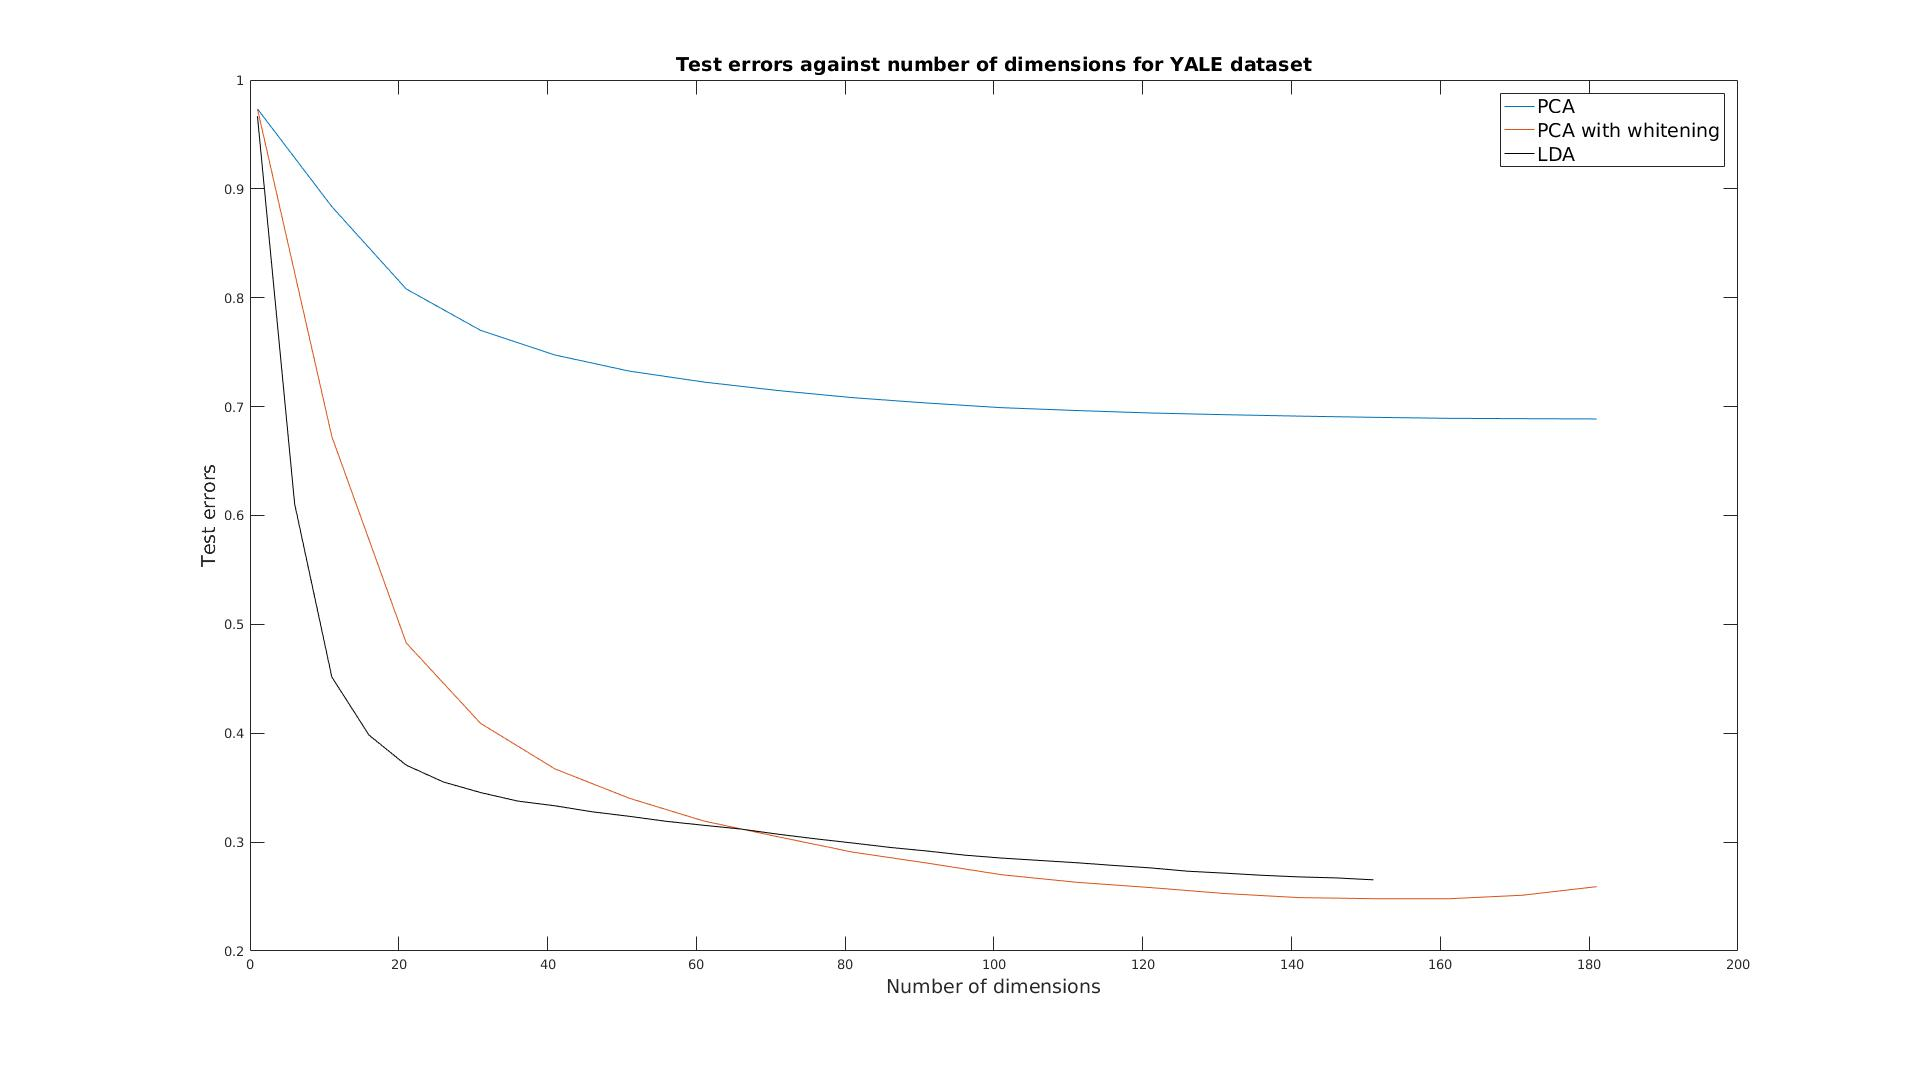
\includegraphics[scale = 0.26]{./figures/YALE.jpg}
  \caption{Graph of test errors against number of dimensions for the YALE dataset.}
  \label{fig:part1YALE}
\end{figure}

\begin{figure}
  \centering
    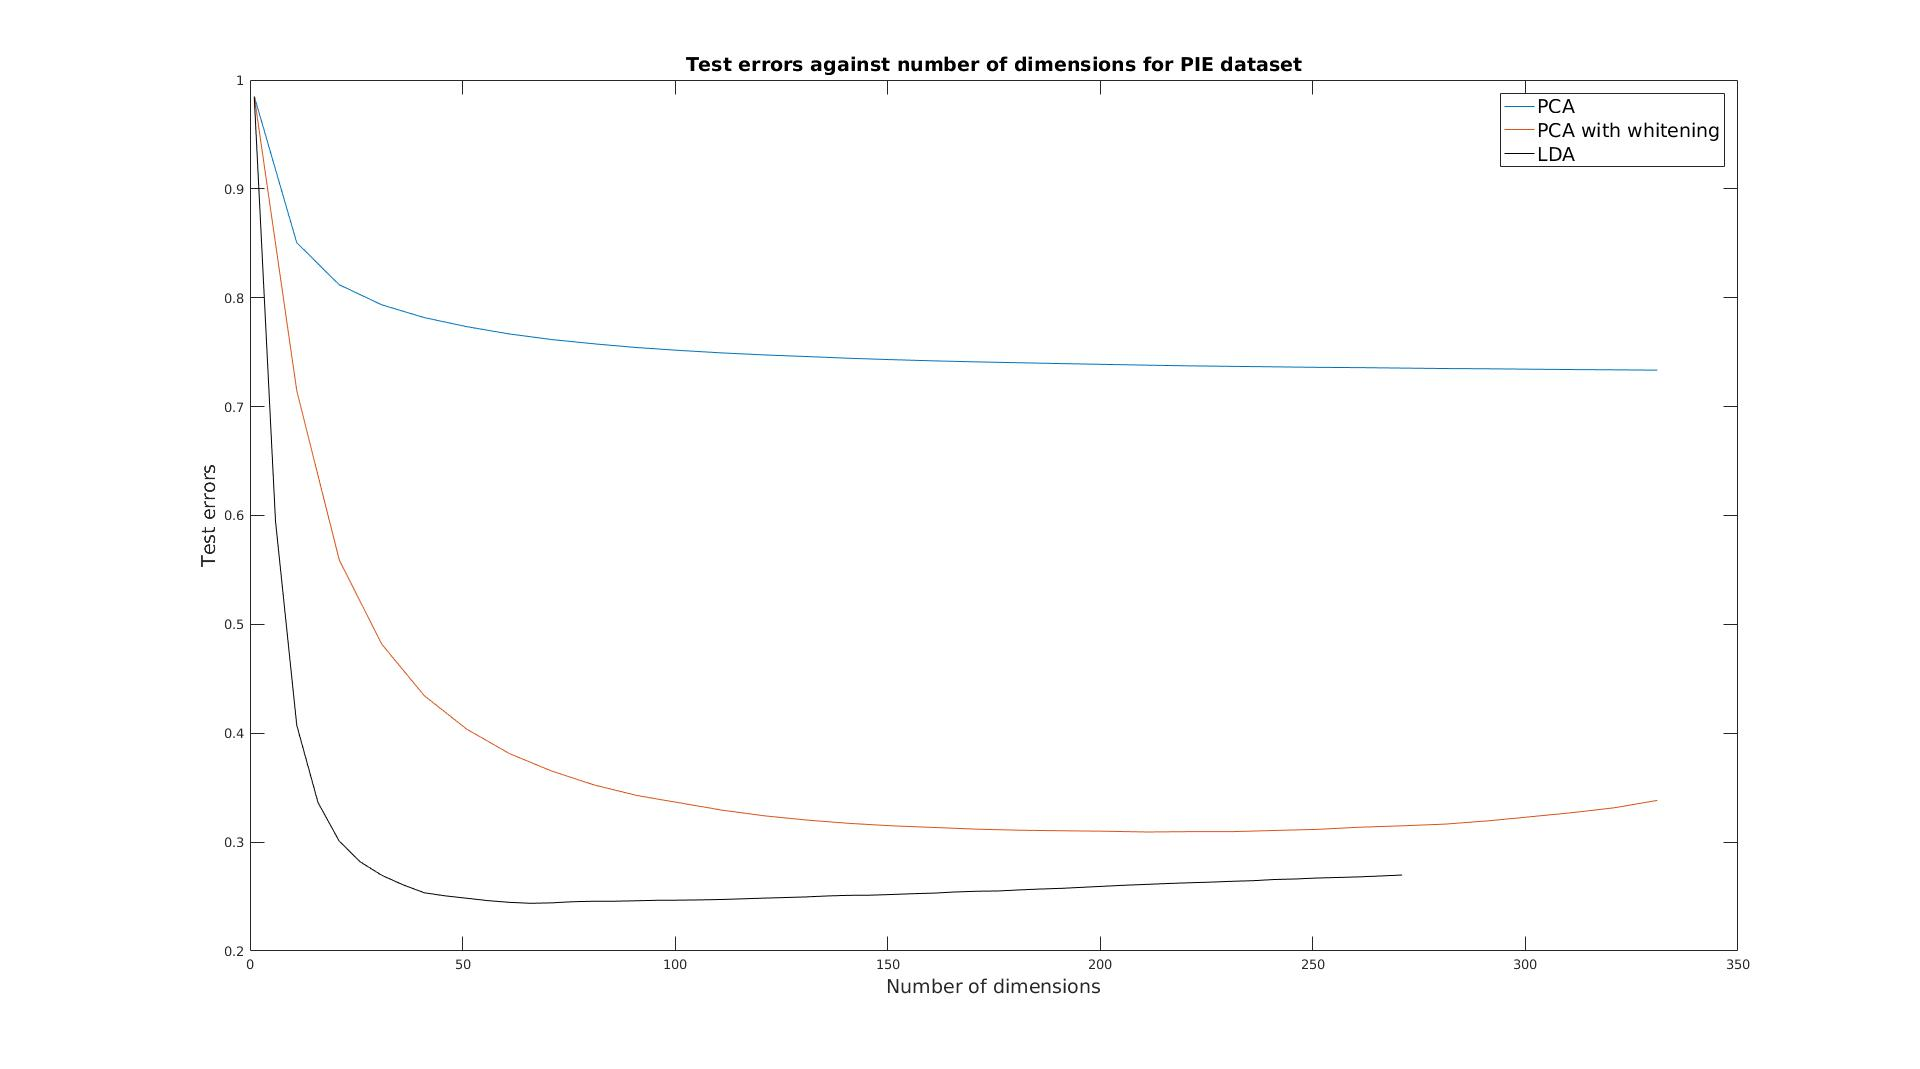
\includegraphics[scale = 0.26]{./figures/PIE.jpg}
  \caption{Graph of test errors against number of dimensions for the PIE dataset.}
  \label{fig:part1PIE}
\end{figure}

\section*{Part II}

\begin{enumerate}[1.)]
\item

The Lagrangian is as follows:
\begin{align}
L(R, \vec a, \xi_i, \lambda, r)
&= R^2 + C \sum_{i=1}^n \xi_i + \sum_{i=1}^n \lambda_i \left[ (\vec x_i - \vec a)\T (\vec x_i-\vec a) - R^2 - \xi_i \right] - \sum_{i=1}^n r_i \xi_i
\end{align}

To find the dual, we need to minimise the Lagrangian with respect to $R$, $\vec a$, and $\xi_i$. We thus differentiate the Lagrangian with respect to these variables:
\begin{align}
\frac{\partial L}{\partial R} &= 2R - 2R \sum_{i=1}^n \lambda_i \overset{!}{=} 0 \quad \Rightarrow \quad 1 - \sum_{i=1}^n \lambda_i = 0 \quad \Rightarrow \quad \sum_{i=1}^n \lambda_i = 1 \label{partTwodldr} \\
\frac{\partial L}{\partial \vec a} &= \sum_{i=1}^n \lambda_i \left[ -2(\vec x_i - \vec a) \right] \overset{!}{=} 0 \quad \Rightarrow \quad \sum_{i=1}^n \lambda_i(\vec x_i - \vec a) = 0 \label{partTwodlda} \\
\frac{\partial L}{\partial \xi_i} &= C - \lambda_i - r_i \overset{!}{=} 0 \quad \Rightarrow \quad C = \lambda_i + r_i \label{partTwodldxi}
\end{align}

Furthermore, from equation \ref{partTwodlda}, we also have the result:
\begin{align}
\sum_{i=1}^n (\lambda_i \vec x_i - \vec a \lambda_i) = 0 \quad \Rightarrow \quad \sum_{i=1}^n (\lambda_i \vec x_i) - \vec a = 0 \quad \Rightarrow \quad \vec a = \sum_{i=1}^n \lambda_i \vec x_i \label{partTwoResultA}
\end{align}
using the result that $\sum_{i=1}^n \lambda_i = 1$ from above. So, using the above equations, we can express the Lagrangian as such:
\begin{align}
L(\lambda)
&= R^2 + \sum_{i=1}^n (\lambda_i + r_i) \xi_i + \lambda_i \sum_{i=1}^n (\vec x_i - \vec a)\T (\vec x_i - \vec a) - R^2 \sum_{i=1}^n \lambda_i - \sum_{i=1}^n \lambda_i \xi_i - \sum_{i=1}^n r_i \xi_i \\
&= R^2 + \sum_{i=1}^n (\lambda_i + r_i) \xi_i + \sum_{i=1}^n \left[ \lambda_i \, (\vec x_i - \vec a)\T (\vec x_i - \vec a) \right] - R^2 - \sum_{i=1}^n (\lambda_i + r_i) \xi_i \\
&= \sum_{i=1}^n \left[ \lambda_i \, (\vec x_i\T - \vec a\T) (\vec x_i - \vec a) \right] \\
&= \sum_{i=1}^n \lambda_i \, \left[ \vec x_i\T \vec x_i - \vec x_i\T \vec a - \vec a\T \vec x_i + \vec a\T \vec a  \right] \\
&= \sum_{i=1}^n \left[ \lambda_i \vec x_i\T \vec x_i - \lambda_i \vec x_i\T \vec a - \lambda_i \vec a\T \vec x_i + \lambda_i \vec a\T \vec a \right] \\
&= \sum_{i=1}^n \left[ \lambda_i \vec x_i\T \vec x_i - \lambda_i \vec x_i\T \vec a - \lambda_i \vec a\T (\vec x_i - \vec a) \right] \\
&= \sum_{i=1}^n \left[ \lambda_i \vec x_i\T \vec x_i - \lambda_i \vec x_i\T \vec a \right] - \vec a\T \underbrace{\sum_{i=1}^n \lambda_i (\vec x_i - \vec a)}_{=0 \text{, from equation \ref{partTwodlda}}}
\end{align}

We also note that, from equation \ref{partTwoResultA}, we have
\begin{align*}
\vec a = \sum_{j=1}^n \lambda_j \vec x_j
\end{align*}

So,
\begin{align}
L(\lambda)
&= \sum_{i=1}^n \left[ \lambda_i \vec x_i\T \vec x_i - \lambda_i \vec x_i\T \vec a \right] \\
&= \sum_{i=1}^n (\lambda_i \vec x_i\T \vec x_i) - \sum_{i=1}^n \lambda_i \vec x_i \T \left( \sum_{j=1}^n \lambda_j \vec x_j \right) \\
&= \sum_{i=1}^n (\lambda_i \vec x_i\T \vec x_i) -  \sum_{i=1}^n \sum_{j=1}^n \lambda_i \vec x_i \T \vec x_j \lambda_j \\
&= \diag (\mat X\T \mat X)\T \lambda - \lambda\T (\mat X\T \mat X) \lambda \\
&= \diag (\mat K_x)\T \vec \lambda - \vec \lambda\T (\mat K_x) \vec \lambda
\end{align}
where $\mat K_x = [\vec x_i\T \vec x_j]$. Hence, we can write the dual as:
\begin{align*}
\max_\vec\lambda \quad &\diag (\mat K_x)\T \vec \lambda - \vec \lambda\T (\mat K_x) \vec \lambda \\
\text{subject to} \quad &\lambda_i \geq 0, \quad 0 \leq \lambda_i \leq C, \quad \text{for } i = 1, \dots , n \\
&\sum_{i=1}^n \lambda_i = 1 \quad \Rightarrow \quad \vec 1\T \vec \lambda = 1
\end{align*}

The second constraint, $0 \leq \lambda_i \leq C$, for $i = 1, \dots , n$ can be derived from equation \ref{partTwodldxi}, which implies that $\lambda_i = C - r_i$. Since $r_i \geq 0$ and $\lambda_i \geq 0$, $r_i$ can only take values from 0 to $C$, inclusive. We then have the constraint, $0 \leq \lambda_i \leq C$.

Furthermore, we can write the above optimisation problem as its equivalent minimisation problem:
\begin{align*}
-\min_\vec\lambda \quad &-\diag (\mat K_x)\T \vec \lambda + \vec \lambda\T (\mat K_x) \vec \lambda \\
\text{subject to} \quad &0 \leq \lambda_i \leq C, \quad \text{for } i = 1, \dots , n \\
&\vec 1\T \vec \lambda = 1
\end{align*}

\item

When using arbitrary positive definite kernels, we can write the above optimisation problem as the following:
\begin{align*}
-\min_\vec\lambda \quad &-\diag (\mat K_x)\T \vec \lambda + \vec \lambda\T (\mat K_x) \vec \lambda \\
\text{subject to} \quad &0 \leq \lambda_i \leq C, \quad \text{for } i = 1, \dots , n \\
&\vec 1\T \vec \lambda = 1
\end{align*}
where $\mat K_x = [k(\vec x_i, \vec x_j)]$ and $k(\vec x_i, \vec x_j) = \phi(\vec x_i)\T \phi (\vec x_j)$ is the kernel.

\item

After identifying the parameters to the MATLAB function \texttt{quadprog} (see MATLAB code), we get an optimal $\vec \lambda^*$ per class, output by the function. We can then substitute the $\vec \lambda^*$ back into the objective function for the dual, to get, say, $-d^*$:

\begin{align*}
-d^* = -\diag (\mat K_x)\T \vec \lambda^* + \vec (\lambda^*) \T (\mat K_x) \vec \lambda^*
\end{align*}

Furthermore, the optimal solution to the primal, $p^*$, is equal to the optimal solution to the dual, $-d^*$, where the negative sign arises from converting our maximisation problem to a minimisation one. We also note that, at the optimal solution, the slack variables, $\xi_i$, go to 0. Hence, keeping $\vec a$ constant, $p^*$ represents the optimal solution to the minimisation problem:
\begin{align*}
R^2 + C \sum_{i=1}^n \xi_i
\end{align*}

As $\xi_i=0$ for all $i = 1, \dots , n$, the optimal $p^*$ is simply the optimal $R^2$. We can thus find the radius of the optimal enclosing hypersphere by taking the square root of $-d^*$. 

We can also find the vector $\vec a_k \in \mathbb{R}^2$, which represents the center of the optimal enclosing hypersphere of class $k$ by:
\begin{align*}
\vec a_k = \sum_{j=1}^n \lambda_j^* \, \vec x_{j,k}
\end{align*}
where $\vec x_{j, k} \in \mathbb{R}^2$ is the $j$th data point of class $k$. The plot of the optimal hyperspheres is in Figure \ref{fig:part2Spheres}.

\begin{figure}
  \centering
    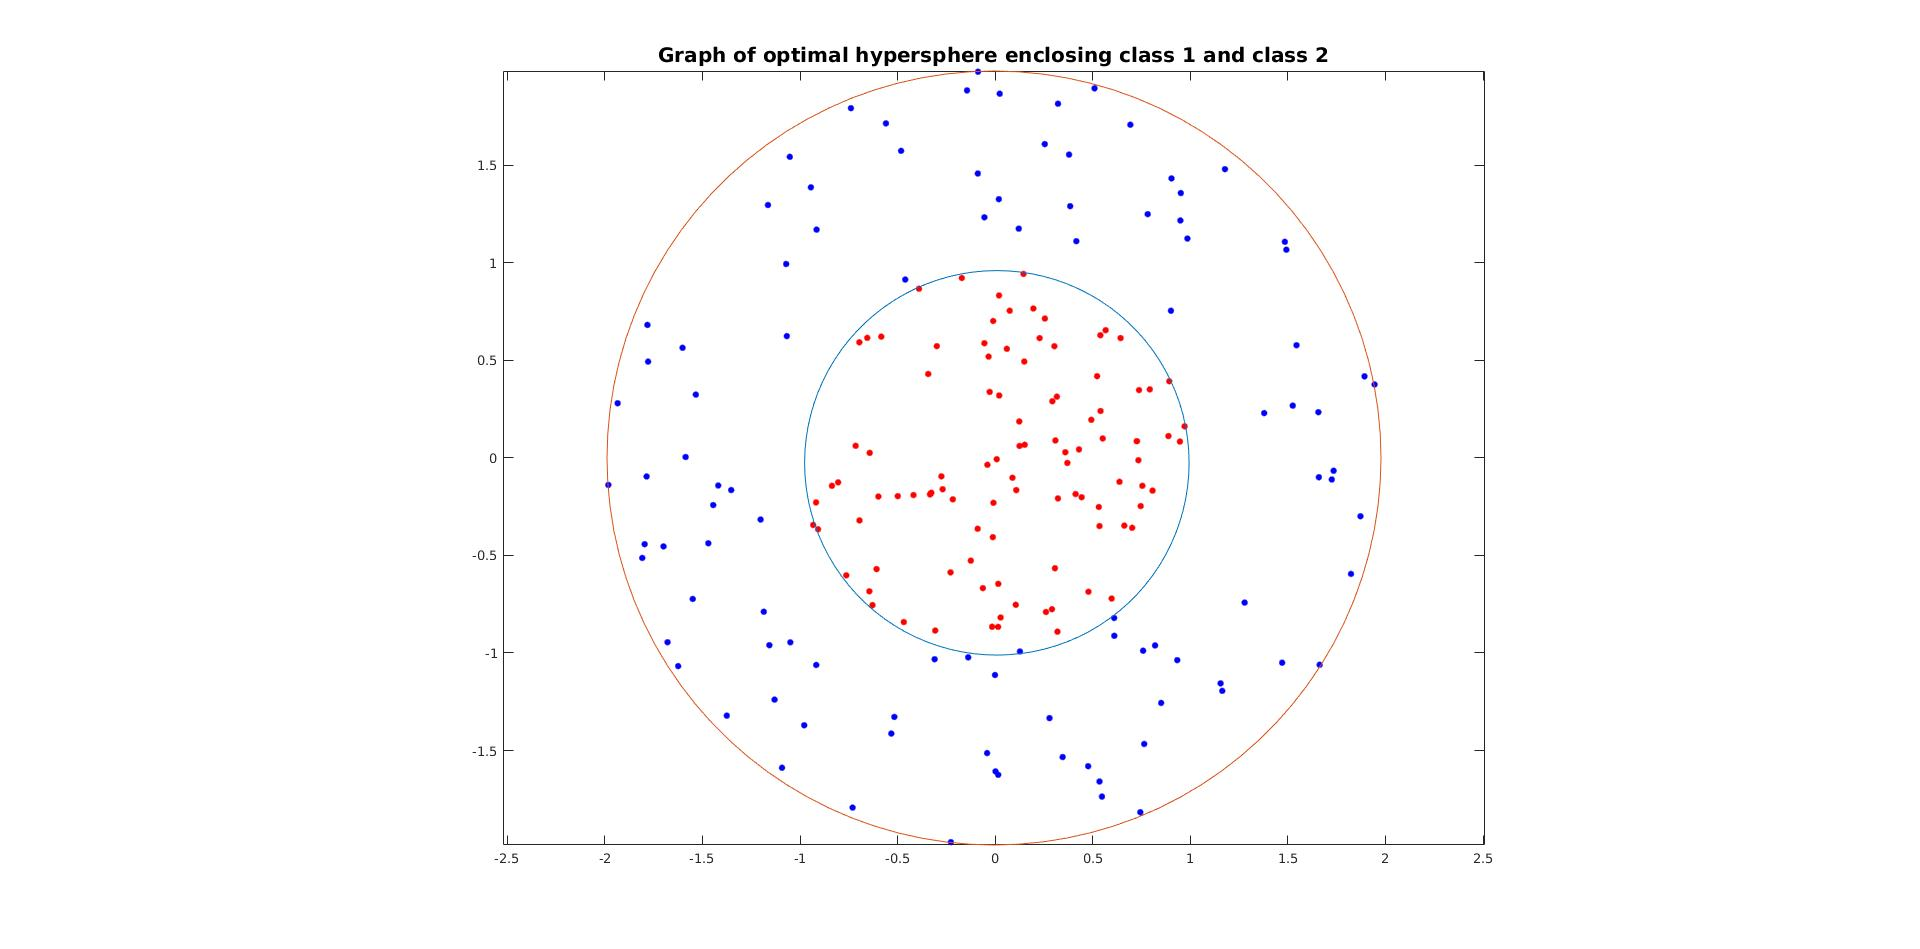
\includegraphics[scale = 0.28]{./figures/sphere.jpg}
  \caption{Plot of data points and the optimal enclosing hyperspheres for each class.}
  \label{fig:part2Spheres}
\end{figure}

\end{enumerate}


\end{document}
